% Name: Seven-segment display
% Description: The seven segments a to g of a digit display, labeled, and the year 2026 lit up from them.
% Tags: seven-segment display, digits, segments, digital electronics

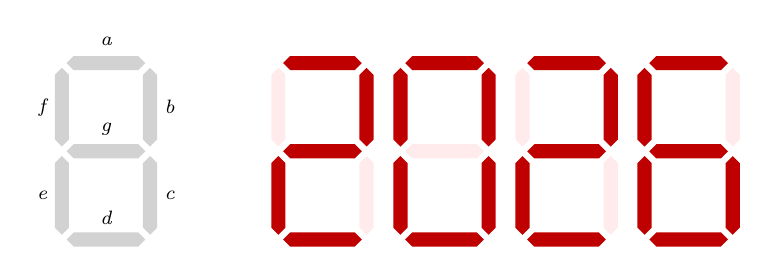
\begin{tikzpicture}[
    seg/.style={draw=#1, line width=0.6pt},
    % A segment of length 1 and thickness 0.18 with pointed ends, horizontal; vertical segments rotate it
    pics/segment/.style={code={\fill (-0.5,0) -- (-0.41,0.09) -- (0.41,0.09) -- (0.5,0) -- (0.41,-0.09) -- (-0.41,-0.09) -- cycle;}}]
  \def\segs{a/0/2.12/0, b/0.56/1.56/90, c/0.56/0.44/90, d/0/-0.12/0, e/-0.56/0.44/90, f/-0.56/1.56/90, g/0/1/0}
  % The template, every segment labeled
  \foreach \s/\x/\y/\r in \segs {
    \pic[gray!35, rotate=\r] at (\x,\y) {segment};
    \node[font=\scriptsize\itshape] at ({\x + (\r == 90 ? (\x > 0 ? 0.25 : -0.25) : 0)}, {\y + (\r == 0 ? 0.28 : 0)}) {\s};
  }
  % 2026: the segments lit for each digit
  \foreach \lit [count=\k] in {{a,b,g,e,d}, {a,b,c,d,e,f}, {a,b,g,e,d}, {a,f,g,e,d,c}} {
    \foreach \s/\x/\y/\r in \segs {
      \def\col{red!8}
      \foreach \l in \lit { \ifx\l\s \gdef\col{red!75!black} \fi }
      \pic[\col, rotate=\r] at ({1.2 + 1.55*\k + \x},\y) {segment};
      \global\let\col\relax
    }
  }
\end{tikzpicture}
